\documentclass[ULlof]{ULrapport}

% Chargement des packages
\usepackage[utf8]{inputenc}
\usepackage[autolanguage]{numprint}
\usepackage{icomma}
\usepackage{multirow}
\usepackage{tabularx}
\usepackage{pbox}
\usepackage{float}
\usepackage{pifont}
\usepackage{pdfpages}

\setcounter{tocdepth}{2}

% Page titre
\TitreProjet{Tableau de hockey interactif}
\TitreRapport{Document de conception -- Remise finale}
\Destinataire{Martin Savoie}
\NomEquipe{The Javangers}
\TableauMembres{
   111\,127\,868  & Jérémie Bolduc & \\\hline
   111\,126\,228  & Simon-Pierre Deschênes & \\\hline
   111\,121\,082  & Émile Grégoire & \\\hline
   111\,130\,693  & Alexandre McCune & \\\hline
}
\DateRemise{18 décembre 2016}


\HistoriqueVersions{
   0.0 & 19 septembre 2016 & Création du document \\\hline
   0.1 & 2 octobre 2016 & Première version après la phase d'inception et le début de l'élaboration \\\hline
   1.0 & 6 novembre 2016 & Version pour la remise 2 \\\hline
   2.0 & 27 novembre 2016 & Version pour la remise 3 \\\hline
   3.0 & 18 décembre 2016 & Version pour la remise finale \\\hline
}

\begin{document}
	
Ce document présente l'évolution du projet VisuaLigue réalisé par l'équipe The Javangers. Le corps du document présente le projet dans l'état actuel. En annexe, vous retrouverez une copie complète des anciens rapports afin de pouvoir voir l'évolution du projet au fil de la session.

\chapter{Vision}
Cette section présente la vision du projet VisuaLigue, un outil de communication de stratégies sportives numérique. La lecture de cette partie est fortement recommandée pour un néophyte du projet, car elle présente le positionnement du produit, une description générale du logiciel et un sommaire des fonctionnalités. Ainsi, la lecture de cette section permet une compréhension globale du projet et une meilleure orientation dans son développement.

\section{Positionnement}
\subsection{Énoncé du problème}
Présentement, la majorité des entraineurs utilisent un tableau blanc avec un arrière-plan de patinoire pour dessiner et expliquer les stratégies. Or, les esquisses sont perdues après chaque entraînement et la visualisation des dessins n'est pas toujours simple.

De plus, le partage et le répertoriage des stratégies sont actuellement difficiles. Généralement, la façon de faire est de photographier le tableau blanc, puis d'envoyer l'image par courriel aux membres intéressés, ou encore de refaire le dessin sur papier ou sur une tablette graphique pour la répertorier.

L'autre problème majeur est la visualisation des stratégies. Souvent, lorsqu'un joueur est présent à une partie, il assiste à l'élaboration de la stratégie et comprend mieux le dessin. Généralement, le mouvement des joueurs est dessiné en temps réel et la gestuelle de l'entraineur est primordiale pour la compréhension. De plus, les trajectoires des joueurs sont souvent effacées pour libérer de l'espace. Or, pour un joueur qui était absent à l'entraînement ou pour un parent qui n'était pas sur la glace lors de l'élaboration de la stratégie, il est souvent difficile de comprendre la stratégie seulement avec le dessin.

\subsection{Opportunité}
Le produit est né d'une demande d'un entraineur de hockey junior qui se plaignait des méthodes traditionnelles d'esquisses de stratégies.

Non seulement un entraineur a manifesté un enthousiasme pour le produit, mais l'Association des entraineurs mineurs du Québec (AEMQ) est aussi intéressée par le produit. D'ailleurs, les spécifications actuelles ont été établies en collaboration avec le président de l'AEMQ.

Outre le milieu du hockey junior, le produit est facilement extensible au milieu professionnel. On remarque notamment l'usage des tableaux blancs dans le domaine professionnel du hockey. De plus, en rendant le logiciel suffisamment flexible, il serait possible d'étendre l'idée pour d'autres sports, notamment le soccer, le football, le volleyball, l'ultimate frisbee, le handball, le kinball, le curling et bien d'autres.

Ce projet pourrait donc avoir des répercussions sur un vaste éventail de sports, dont certaines ligues professionnelles qui engrangent des quantités impressionnantes d'argent. Plusieurs de ces sports sont présents un peu partout dans le monde, tant au niveau amateur que professionnel. La démarcation du produit pourrait d'ailleurs se faire à de nombreux événements sportifs tels que des tournois, des championnats internationaux et même les Jeux olympiques.

\subsection{Alternatives et compétition}
Les alternatives présentement sur le marché représentent davantage des outils de dessin sur ordinateur. Notamment, le logiciel ConceptDraw PRO\footnote{\url{http://www.conceptdraw.com/How-To-Guide/ice-hockey-diagram-defensive-strategy-neutral-zone-trap}} offre des extensions pour le dessin de stratégies de hockey.

De nombreux logiciels sont disponibles sur les tablettes pour le dessin. Certains de ces logiciels permettent la projection simultanée pour une meilleure visualisation par les joueurs.

Or, ces solutions permettent seulement de réaliser des images statiques. Celles-ci sont plus faciles à répertorier considérant leur support numérique. Toutefois, le problème de visualisation est toujours présent. Il est difficile de visualiser la stratégie à partir d'une image fixe.

\subsection{Résumé du produit}
VisuaLigue est une application qui permet la création et la visualisation de stratégies sportives. Un entraineur peut donc facilement placer les joueurs, les obstacles et les objets sur un terrain virtuel. Ces éléments peuvent ensuite être modifiés facilement grâce à une interface utilisateur conviviale. Le logiciel permet aussi de visualiser la stratégie de manière dynamique. Ainsi, l'entraineur peut démarrer la visualisation et montrer à tout le monde le déplacement des joueurs en temps réel. Il peut aussi mettre la visualisation sur pause, avancer, reculer et regarder image par image. Finalement, l'application permet la sauvegarde des jeux pour permettre le partage et le répertoriage.

Le tableau \ref{t:fonctionnalites} présente un sommaire non exhaustif des fonctionnalités du logiciel ainsi que les avantages offerts pour les parties prenantes.

\begin{table}[h]
	\begin{tabular}{|p{6cm}|p{8cm}|}
		\hline
		\bfseries{Fonctionnalité}              & \bfseries{Avantage pour les parties prenantes} \\\hline
		Création de stratégies numériquement   & Facile à partager, schéma plus clair, notation standardisée \\\hline
		Visualisation des stratégies (lecture, pause, avancer, reculer, image par image, etc.) & Meilleure compréhension des joueurs, surtout s'ils n'étaient pas présents lors de l'élaboration de la stratégie \\\hline
		Création de nouveaux types de sports   & Plus grande flexibilité pour les entraineurs. Extension du projet vers des sports autres que le hockey \\\hline
		Création de nouveaux types d'obstacles & Flexibilité du logiciel pour différents types d'entraînements \\
		\hline
	\end{tabular}
	\caption{Fonctionnalités et avantages pour les parties prenantes}
\end{table}

D'autres fonctionnalités plus techniques ont été énoncées durant les discussions. Les points suivants ont notamment été soulevés:
\begin{itemize}
	\item Fonctionnalité d'annuler/rétablir
	\item Exporter les stratégies sous un format d'image (PNG, JPEG, etc.)
	\item Zoom
	\item Affichage des coordonnées de la souris lors du déplacement sur l'aire de jeu
	\item Option pour montrer/cacher le rôle des joueurs
\end{itemize}

\chapter{Images de l'application}

Cette section présente des images tirées de l'application.

%\begin{figure}[H]
%	\centering
%	\includegraphics[width=\textwidth]{{"fig/diagrams3/Diagramme etats joueur"}.png}
%	\caption{Diagramme d'états pour un joueur}
%\end{figure}

%\begin{figure}[H]
%	\centering
%	\includegraphics[width=\textwidth]{{"fig/diagrams3/Diagramme etats rondelle"}.png}
%	\caption{Diagramme d'états pour la rondelle}
%\end{figure}

\chapter{Modèle du domaine}

Cette section présente le modèle du domaine, une vision haut-niveau de l'organisation de l'application.

\begin{figure}[H]
	\centering
	\includegraphics[width=4in]{{"fig/diagrams4/Modele du domaine"}.png}
	\caption{Modèle du domaine de VisuaLigue}
\end{figure}

\chapter{Diagramme de classe}

Cette section présente le diagramme de classe mis à jour pour le code tel que remis dans le livrable final.

\begin{figure}[H]
	\centering
	\includegraphics[width=\textwidth]{{"fig/diagrams4/Diagramme de classe"}.png}
	\caption{Diagramme de classe de conception avec packages}
\end{figure}

\chapter{Points forts et points faibles de l'application}

Cette section présente les points forts et les points faibles de l'application. Il sera question des améliorations possibles afin que l'application puisse être utilisée en contexte réel ainsi que de ce qui pourrait la rendre plus efficace.

Tout d'abord, parmi les points forts de notre application, le plus important est la flexibilité vis-à-vis les modes d'éditions. En effet, notre application permet de changer de mode d'édition très aisément. De plus, en raison de l'interpolation des positions qui est faite lors du visionnement d'une stratégie, les trajectoires des joueurs sont très fluides. Il est donc très facile pour l'utilisateur de modifier une stratégie et d'avoir un résultat de bonne qualité.

Pour ce qui est des points faibles de notre application, le plus prédominant serait la présence de quelques bugs. Malgré qu'ils soient mineurs, certains malfonctionnements ont pu être observés. Plusieurs d'entre eux n'ont cependant pas d'impact réel sur l'application. Par exemple, il arrive qu'il y ait une erreur d'affichage et que le curseur de la ligne du temps pointe entre deux images. Un autre exemple de malfonctionnement est l'édition en temps réel de l'orientation. Il n'y a pas d'erreur, mais c'est plutôt difficile de l'éditer exactement selon nos désirs. Malgré tout, rien n'empêche de réaliser la tâche demandée.

Ainsi, afin que l'application puisse être utilisée dans un contexte réel, il suffirait seulement de régler les quelques malfonctionnements décrits ci-dessus, car elle répond tout à fait à la demande de manière efficace tout en offrant une interface sobre et épurée.

Finalement, afin de rendre l'application plus efficace, il serait assez difficile d'améliorer les fonctionnalités existantes, car elles répondent assez bien à leur rôle. Ainsi, pour que ce soit plus efficace, il faudrait plutôt implémenter de nouvelles fonctionnalités. Par exemple, l'exportation des stratégies en vidéo ou bien l'envoi de stratégies par courriel pourraient être des fonctionnalités tout à fait intéressantes pour rendre l'application plus polyvalente et efficace.

\chapter{Plan de travail}

La figure \ref{fig:gantt} présente l'échéancier du projet.

\begin{figure}[p]
	\centering
	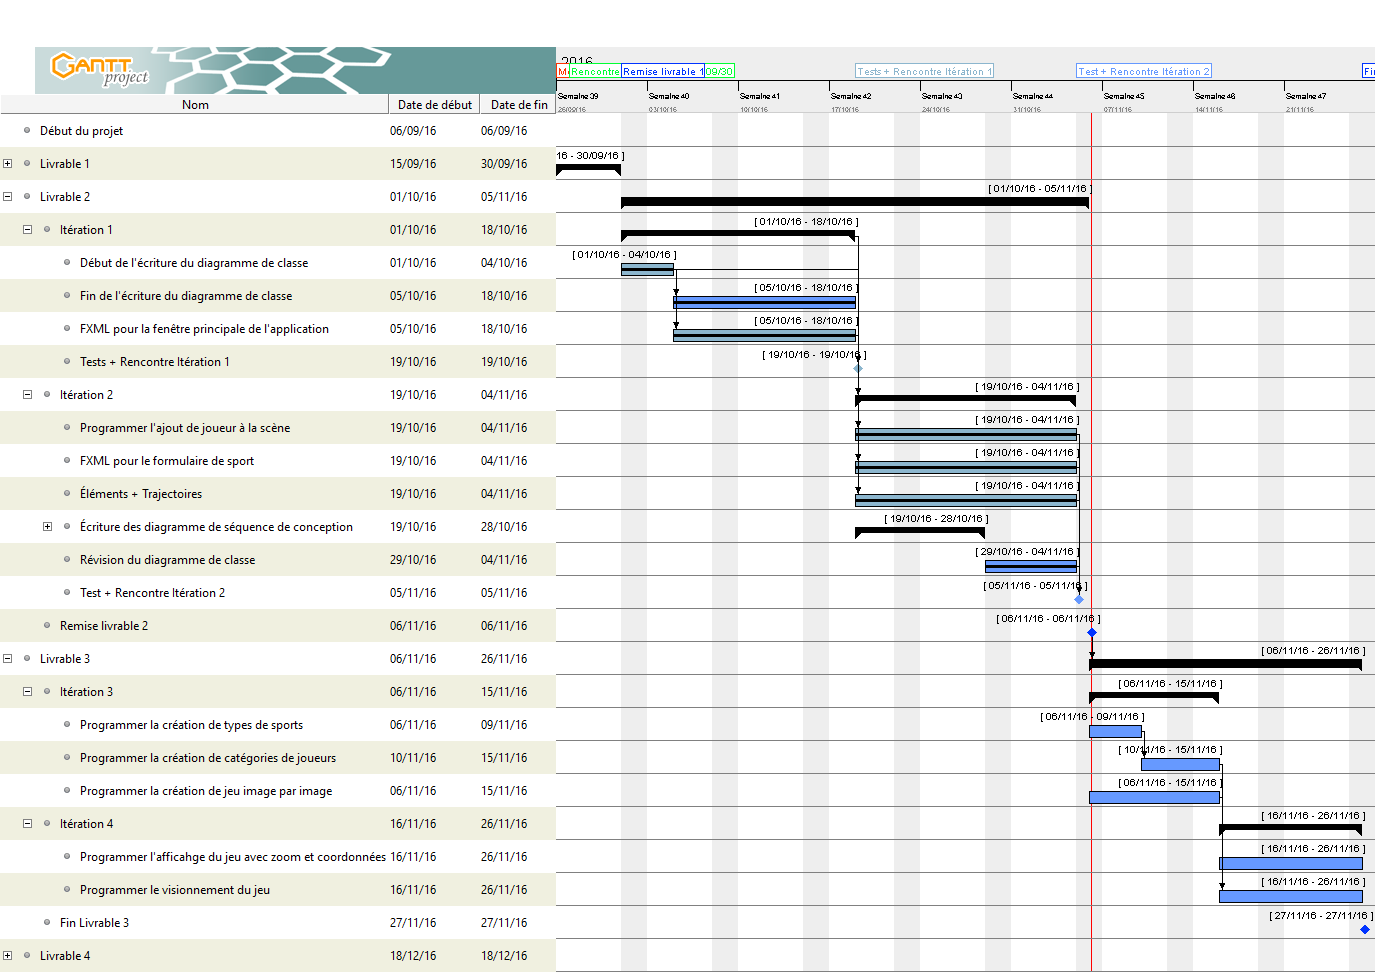
\includegraphics[scale=0.35, angle=90]{fig/diagrams4/gantt.png}
	\caption{Échéancier du projet}
	\label{fig:gantt}
\end{figure}

\appendix

\chapter{Remise 3}
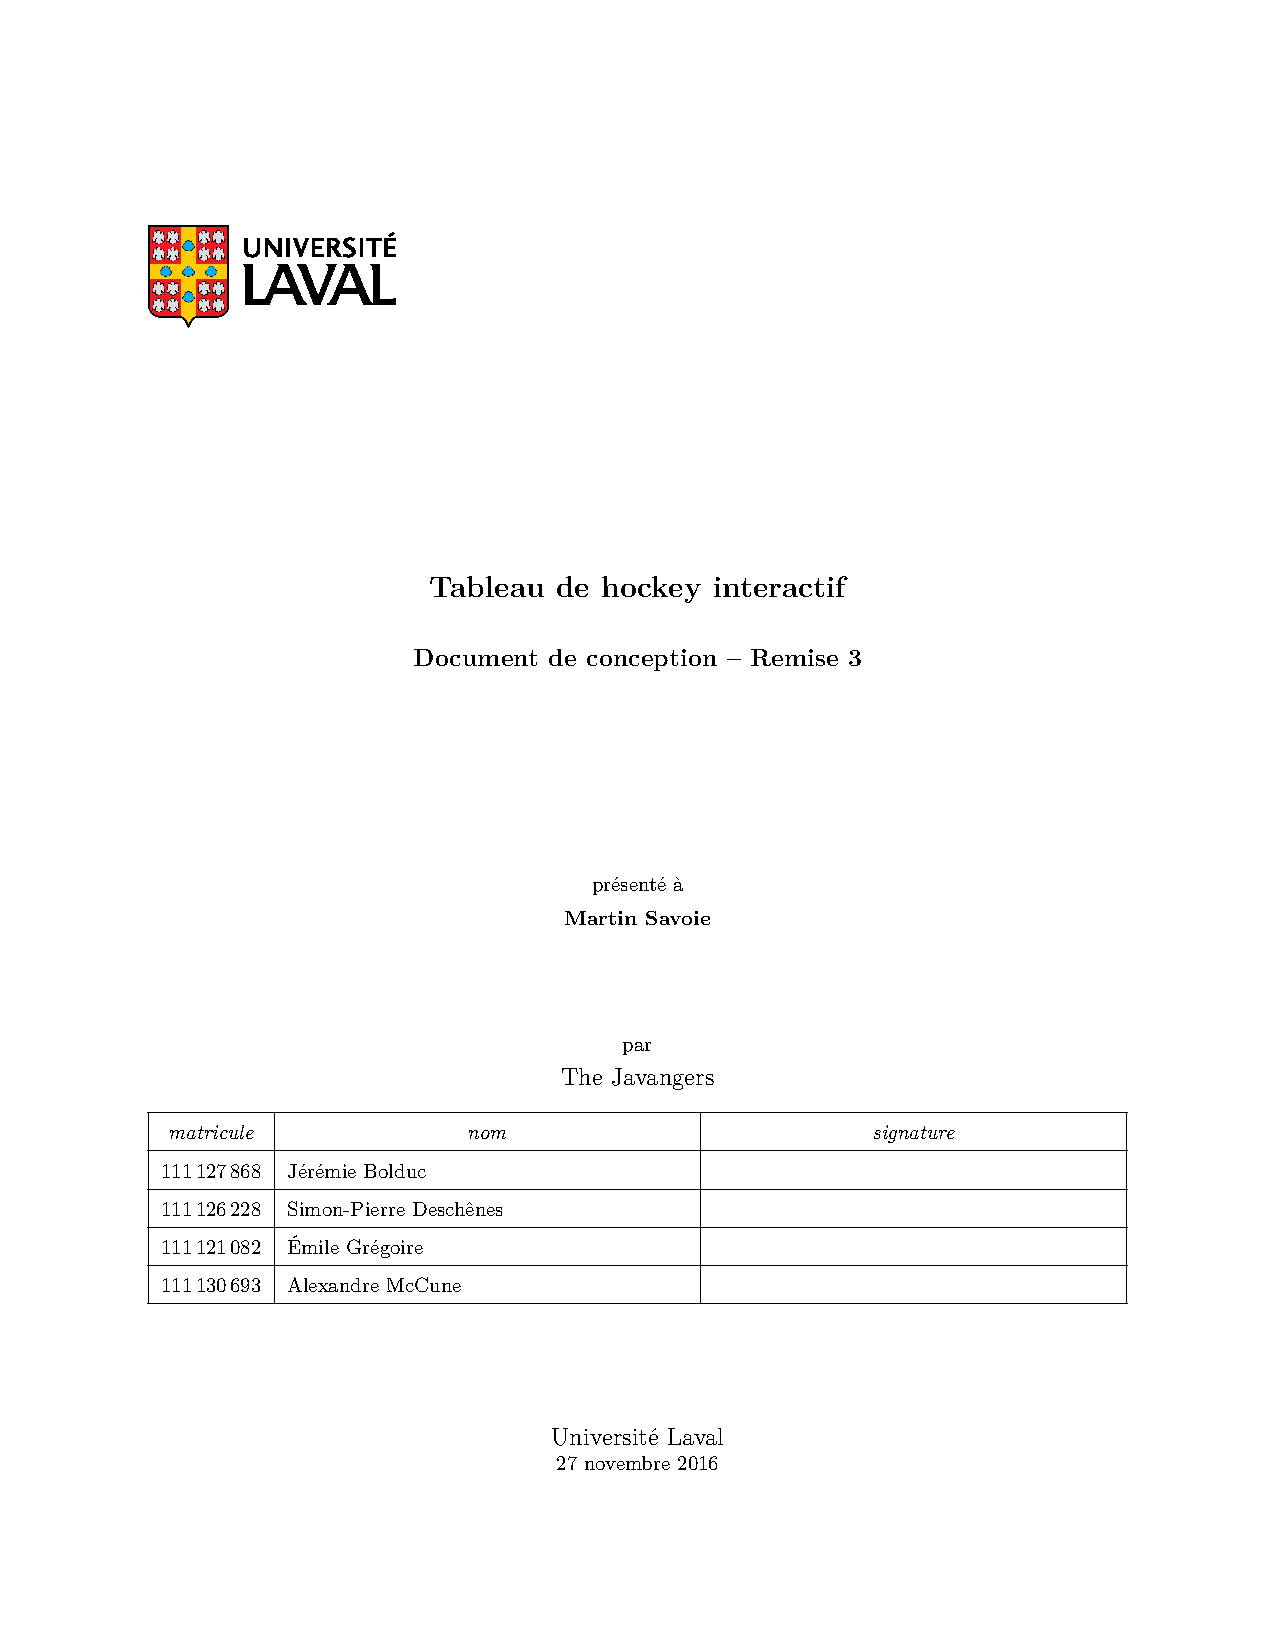
\includepdf[pages=-]{old/Remise3}

\chapter{Remise 2}
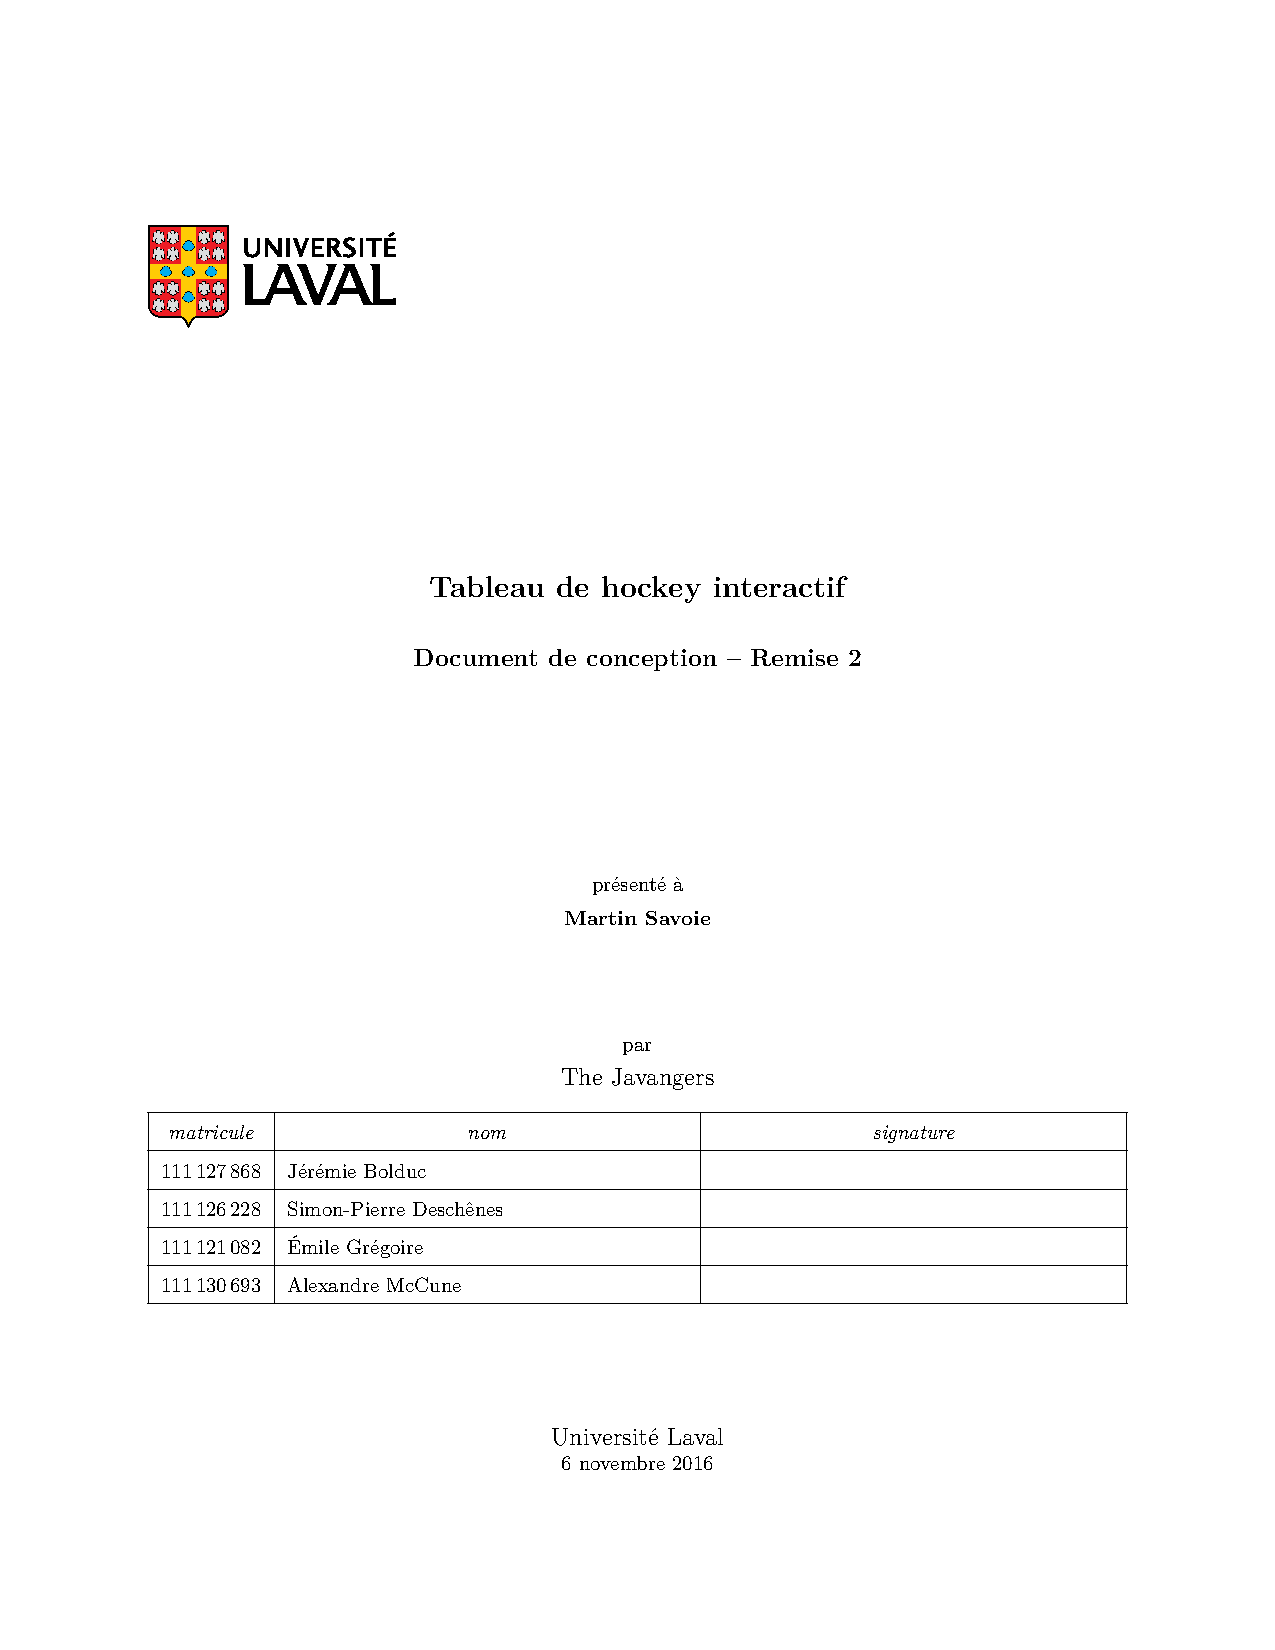
\includepdf[pages=-]{old/Remise2}

\chapter{Remise 1}
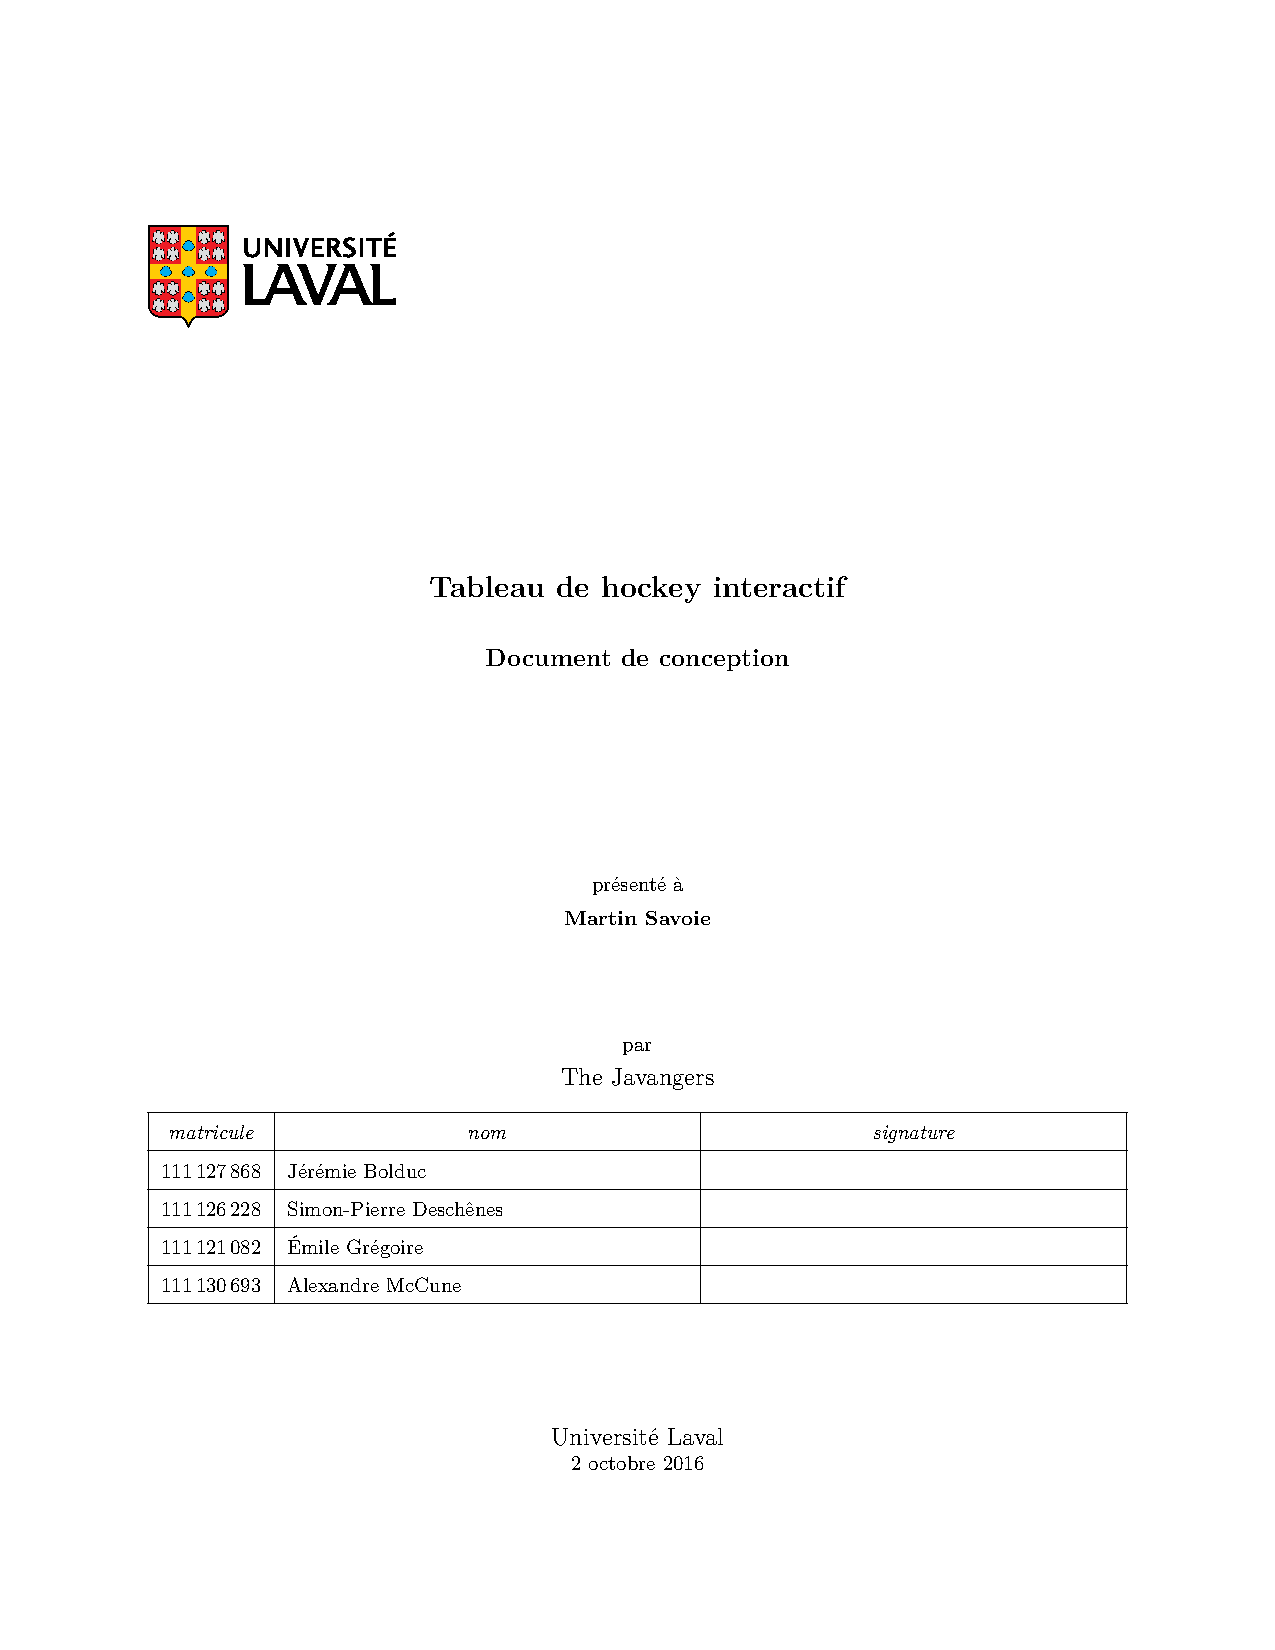
\includepdf[pages=-]{old/Remise1}

\end{document}
